\section{Data Samples.}
	
	The detector was placed in different positions respect to the beam, the main places are shown in  Figure \ref{figure:zones}.
	Furthermore, to study the uniformity of charge and efficiency along the components it was necessary to take more runs to complete this analysis. %
	The beam momentum was set at 1 GeV/c for the general study of the components
	%; at 1.5 GeV/c for the pixel detector run;
	and another set at 1.5, 2 and 6 GeV/c for hitting at the center of the plastic scintillator.
	%
	Unlike the use of the FEE in the ALICE environment, in T10 a synchronization signal with the particles source 
	is not available, and the 	events occurs randomly, therefore we have to define a reference for time, we 
	mainly use T0-end detector to perform that function. %
	Is worth to mention that the signal from the T0s was changed from NIM to TTL level having a constant width and 
	the charge was not measured. %
	The	width distribution of the T0-start %(left from Figure \ref{figure:widthClean}) 
	is not as expected, some events are outside from a narrow distribution; meanwhile the T0-end distribution
	%(right from Figure \ref{figure:widthClean}) 
	shows a single narrow peak and to avoid that noise we select the events in a time window between 13 and 17 ns 
	in T0-start. %
	
	\begin{figure}[ht!]
		\begin{center}
			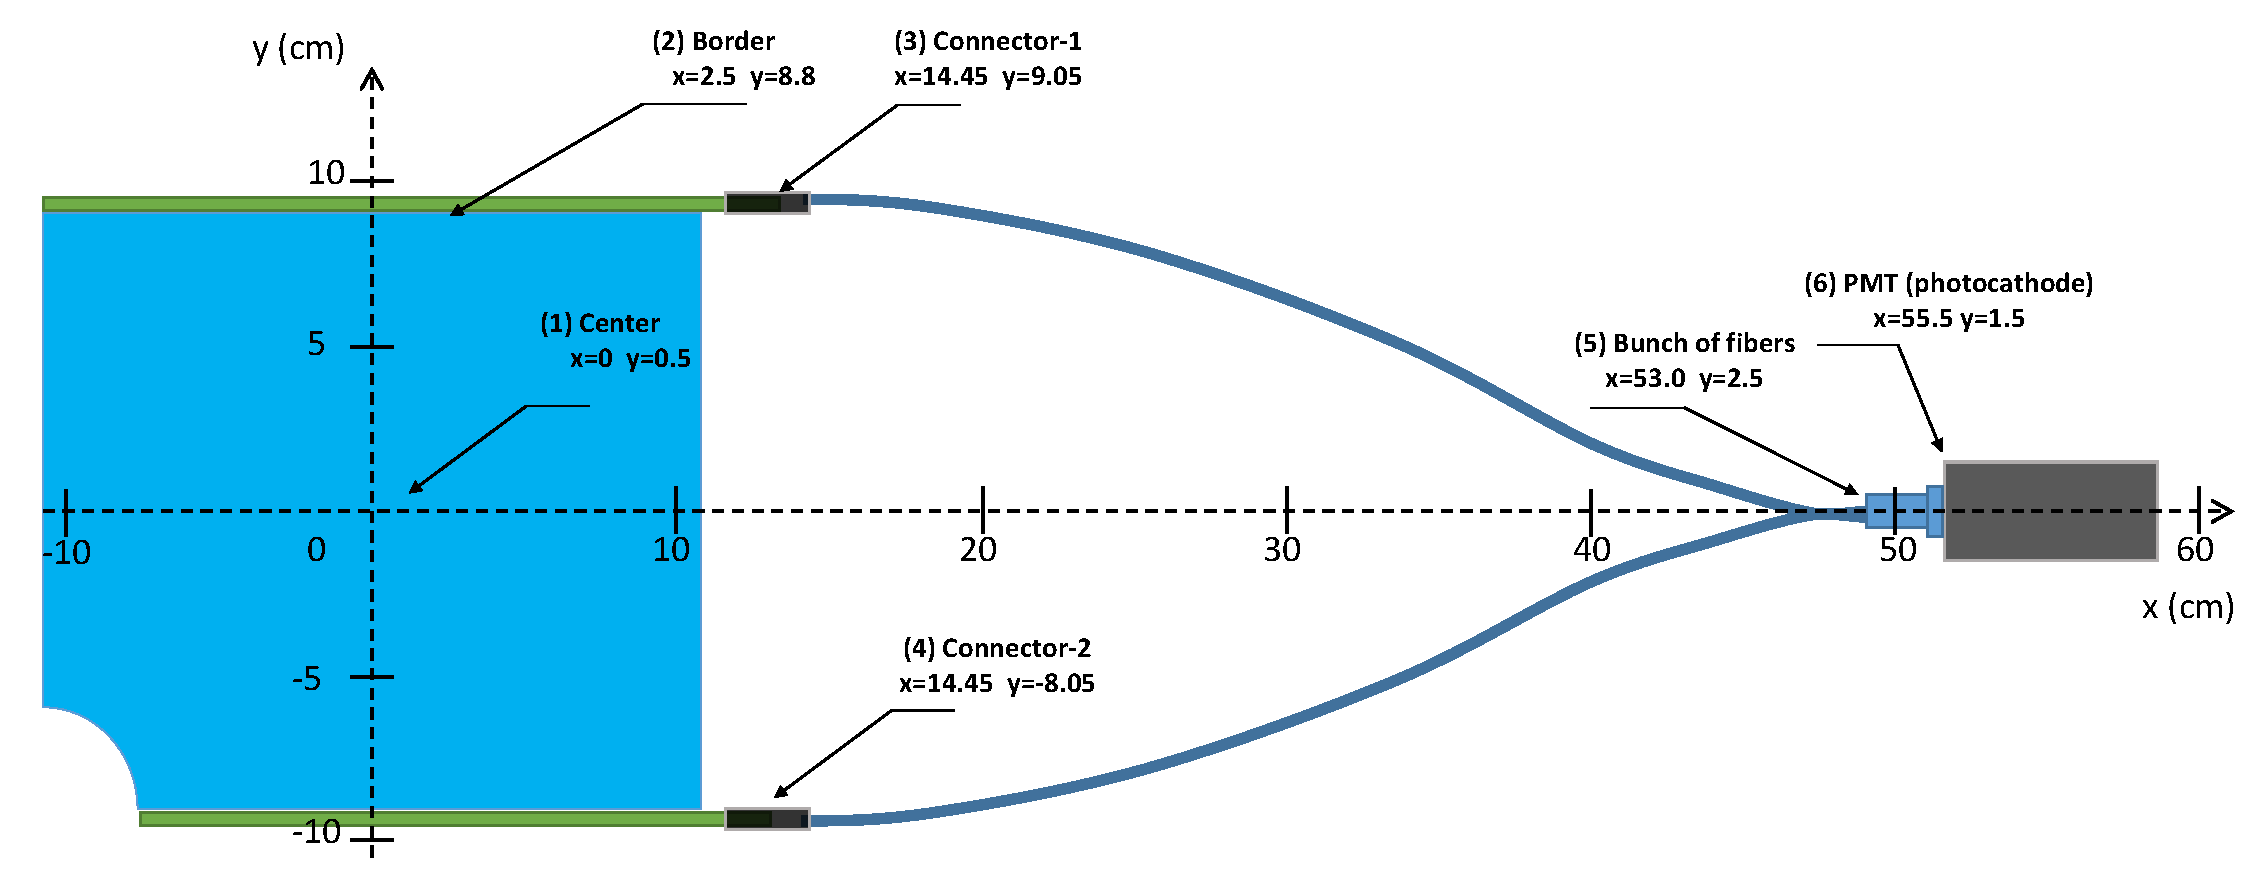
\includegraphics[scale=0.40]{./images/AD-2D.pdf}
			\caption{Scheme of positions respect to the plastic scintillator center and 
				beam conditions for the main point of the detector.%, including the pixel detector.
			}
			\label{figure:zones}
		\end{center}
	\end{figure}

All those cleaning criteria were used along in furthers studies. Some other specific cleaning techniques
were applied depending on the particular characteristics of the analysis.
